\chapter{Heralded Quantum Gates with Integrated Error Detection}
\label{ch:Borregaard_PRL2015}
%%%%%%%%%%%%%%%%%%%%%%%%%%%%%%%%%%%%%%%%%%%%%%%%

\section{Introduction}
%From \cite{Borregaard2015a}

Exploiting quantum systems for information processing offers many potential
advantages over classical information processing like highly secure quantum
networks~\cite{cirac,kimble, duan3} and powerful quantum
computers~\cite{ladd,shor,feynman}. One of the main challenges for the
realization of functional quantum computers is to perform gates with
sufficiently high quality so that the remaining errors can be suppressed by
error correction codes, which makes the computation fault tolerant
\cite{knill2}. At the same time, applications to long distance quantum
communication can be enabled by quantum repeaters, which combine probabilistic
entanglement generation over short distances with subsequent entanglement
connection steps \cite{duan3}. For these protocols, the probabilistic nature of
the entanglement generation is acceptable, but it is essential that high
fidelity entanglement is achieved conditioned on a heralding measurement.
Experimentally, such high fidelity entanglement is often much easier to
implement and may be realized in situations where it is impossible to perform
any quantum operations deterministically. Here we introduce a similar concept
for gate operations and develop the concept of  heralded quantum gates  with
integrated error detection. In the resulting gate, the infidelity, which would
be present for a deterministic gate is converted into a failure probability,
which is heralded by an auxiliary atom. Once successful, the resulting gate can
have an arbitrarily small error. Such heralded gates could facilitate fault
tolerant quantum computation since detectable errors may be easier to correct
than undetectable errors~\cite{grassi,ralph05,varnava}.  Alternatively it can be
directly incorporated into quantum repeater architectures for long distance
quantum communication.

Optical cavities are ideal for conversion between the stationary gate qubits and
flying qubits (photons), which is fundamental for quantum networks \cite{ritter,
Komar2014, acin}. Quantum gates can, in principle, also be directly implemented in
optical cavities \cite{pellizari}, but the experimental requirements for this
are very challenging due to spontaneous emission and cavity loss. The essential
parameter quantifying this is the cooperativity of the atom-cavity system, $C$.
It has been argued that directly implementing gates in optical cavities leads to
a poor error scaling $1-F\propto1/\sqrt{C}$, where $F$ is the fidelity of the
gate \cite{kastoryano, Anders2prl}. However, as a result of the integrated error
detection, the heralded gates that we propose exhibit high fidelities when
successful. This enables efficient entanglement swapping and removes the
necessity of intermediate entanglement purification in quantum repeaters thus
increasing the distribution rate significantly. Compared to using other
deterministic, cavity based gates, an increase in the rate of up to two orders
of magnitude can be achieved for modest cooperativities ($<100$) and a distance
of 1000 km \cite{Borregaard2015b}.

\section{Heralding gate}

The basic idea is to use a heralding auxiliary atom in addition to qubit atoms
in the same cavity. One of the atomic qubit states, e.g., state $\ket{1}$
couples to the cavity mode while $\ket{0}$ is completely uncoupled (see
\reffig{fig:levels}(a)). Such a system has previously been considered for two-qubit
gates~\cite{duan1, DuanPRL2004, Anders1prl, Anders2prl,ritter2014}, multi-qubit
gates~\cite{duan1,zheng} and photon routing~\cite{Tiecke}.
If any of the qubit atoms is in state $\ket{1}$ the cavity resonance is shifted
compared to the bare cavity mode, which can be exploited to make a gate between
two or more qubits by reflecting single photons off the cavity \cite{duan1}. The
efficiency of such schemes, however, is limited by photon losses, inefficient
detectors and non-ideal single photon sources \cite{Tiecke,ritter2014}. We
circumvent these problems by introducing an auxiliary atom in the cavity to
serve as both an intra-cavity photon source and a detector. As opposed to
previous heralded gates in optical cavities, which relied on the null detection
of photons leaving the cavity \cite{pachos,beige, vitali}, the final heralding
measurement on the atom can then be performed very efficiently.

In our approach, the auxiliary atom has two metastable states $\ket{g},\ket{f}$,
which can be coupled through an excited state $\ket{E}$ (see
\reffig{fig:levels}(a)). We assume the $\ket{E}\leftrightarrow\ket{f}$ transition
to be energetically close to the cavity frequency and to be a nearly closed
transition,  so that we need to drive the $\ket{g}\to \ket{E}$ transition, e.g
with a two-photon process, (see below).
The gate can be understood through the phase evolution imposed on the atoms. We
consider adiabatic excitation of the auxiliary control atom via Stimulated Raman
Adiabatic Passage~\cite{stirap,stirap2}, driven by an external driving pulse
with Rabi frequency $\Omega(t)$ and a coupling to the cavity photon $g_{f}$. In
the case when all the qubit atoms are in the non-coupled states $|00..0\rangle$,
an adiabatic excitation will result in a dark state $\sim g_{f} \ket{0,g}
-\Omega \ket{1,f}$ with zero energy and vanishing phase. Here the number refers
to the number of cavity photons.  However, the qubit states $\Psi$ with at least
one of the qubit atoms in the coupled state, results in a cavity-induced shift
of the state $|1,f, \Psi\rangle$, which in turn, causes an AC Stark shift and
dynamical phase to be imprinted into the $|g,\Psi\rangle$ state after the
driving pulse is turned off. All states but the completely uncoupled qubit state
$|00...0\rangle$ will thus acquire a phase, the magnitude of which depends on
the length of the driving pulse. With an appropriate pulse length and simple
single qubit rotations, we can use this to realize a general $N$-qubit Toffoli
gate or a control-phase (CZ) gate.

Naively, the gates will be limited by errors originating from cavity decay and
spontaneous emission from the atoms, which carry away information about the
qubit state. These errors are, however, detectable since the auxiliary atom will
be trapped in state $\ket{f}$ if either a cavity excitation or an atomic
excitation is lost. Conditioning on detecting the auxiliary atom in state
$\ket{g}$ at the end of the gate thus rules out the possibility of any
dissipative quantum jumps having occurred during the gate. As a result, the
conditional fidelity of the gate is greatly enhanced at the modest cost of a
finite but potentially low failure probability.
\begin{figure}
\centering
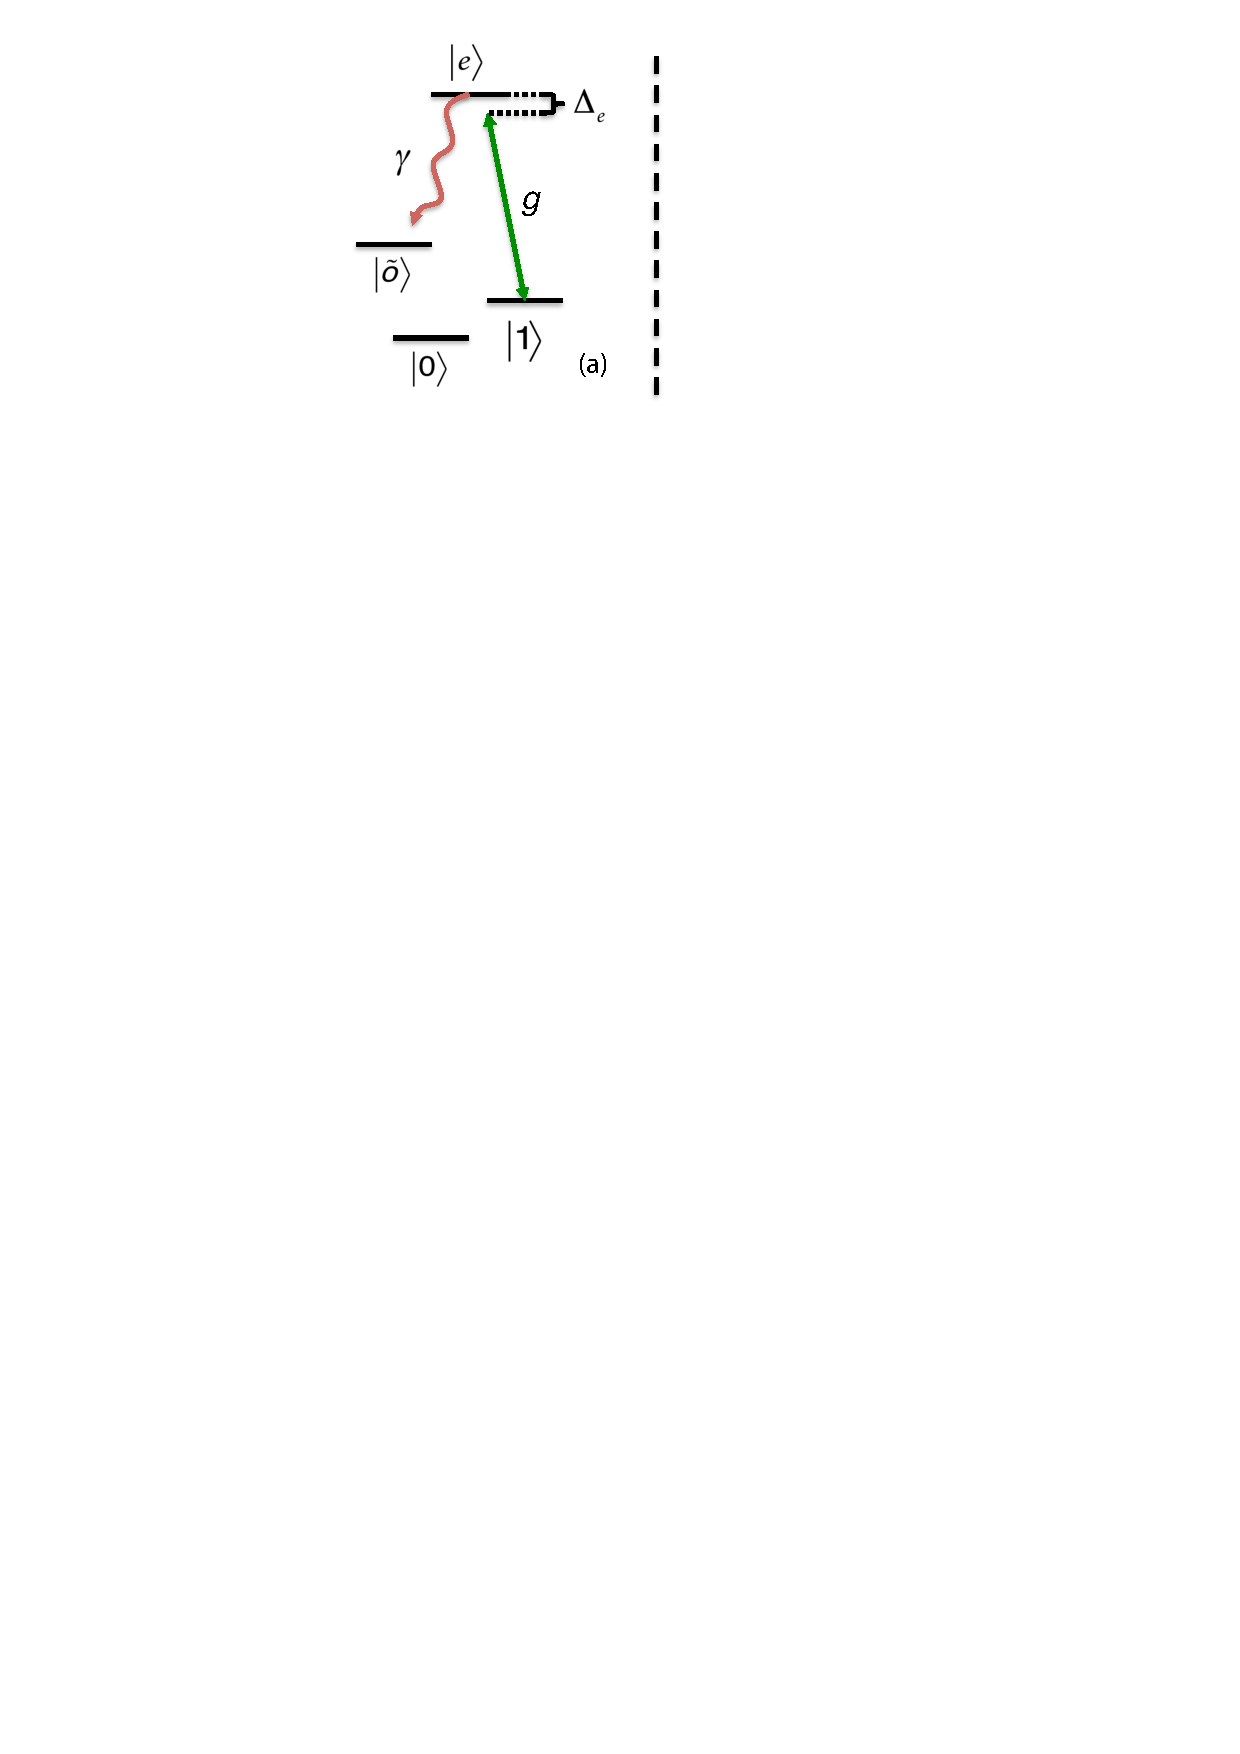
\includegraphics[width=0.35\textwidth]{./figs_Borregaard_PRL2015/figure1a} 
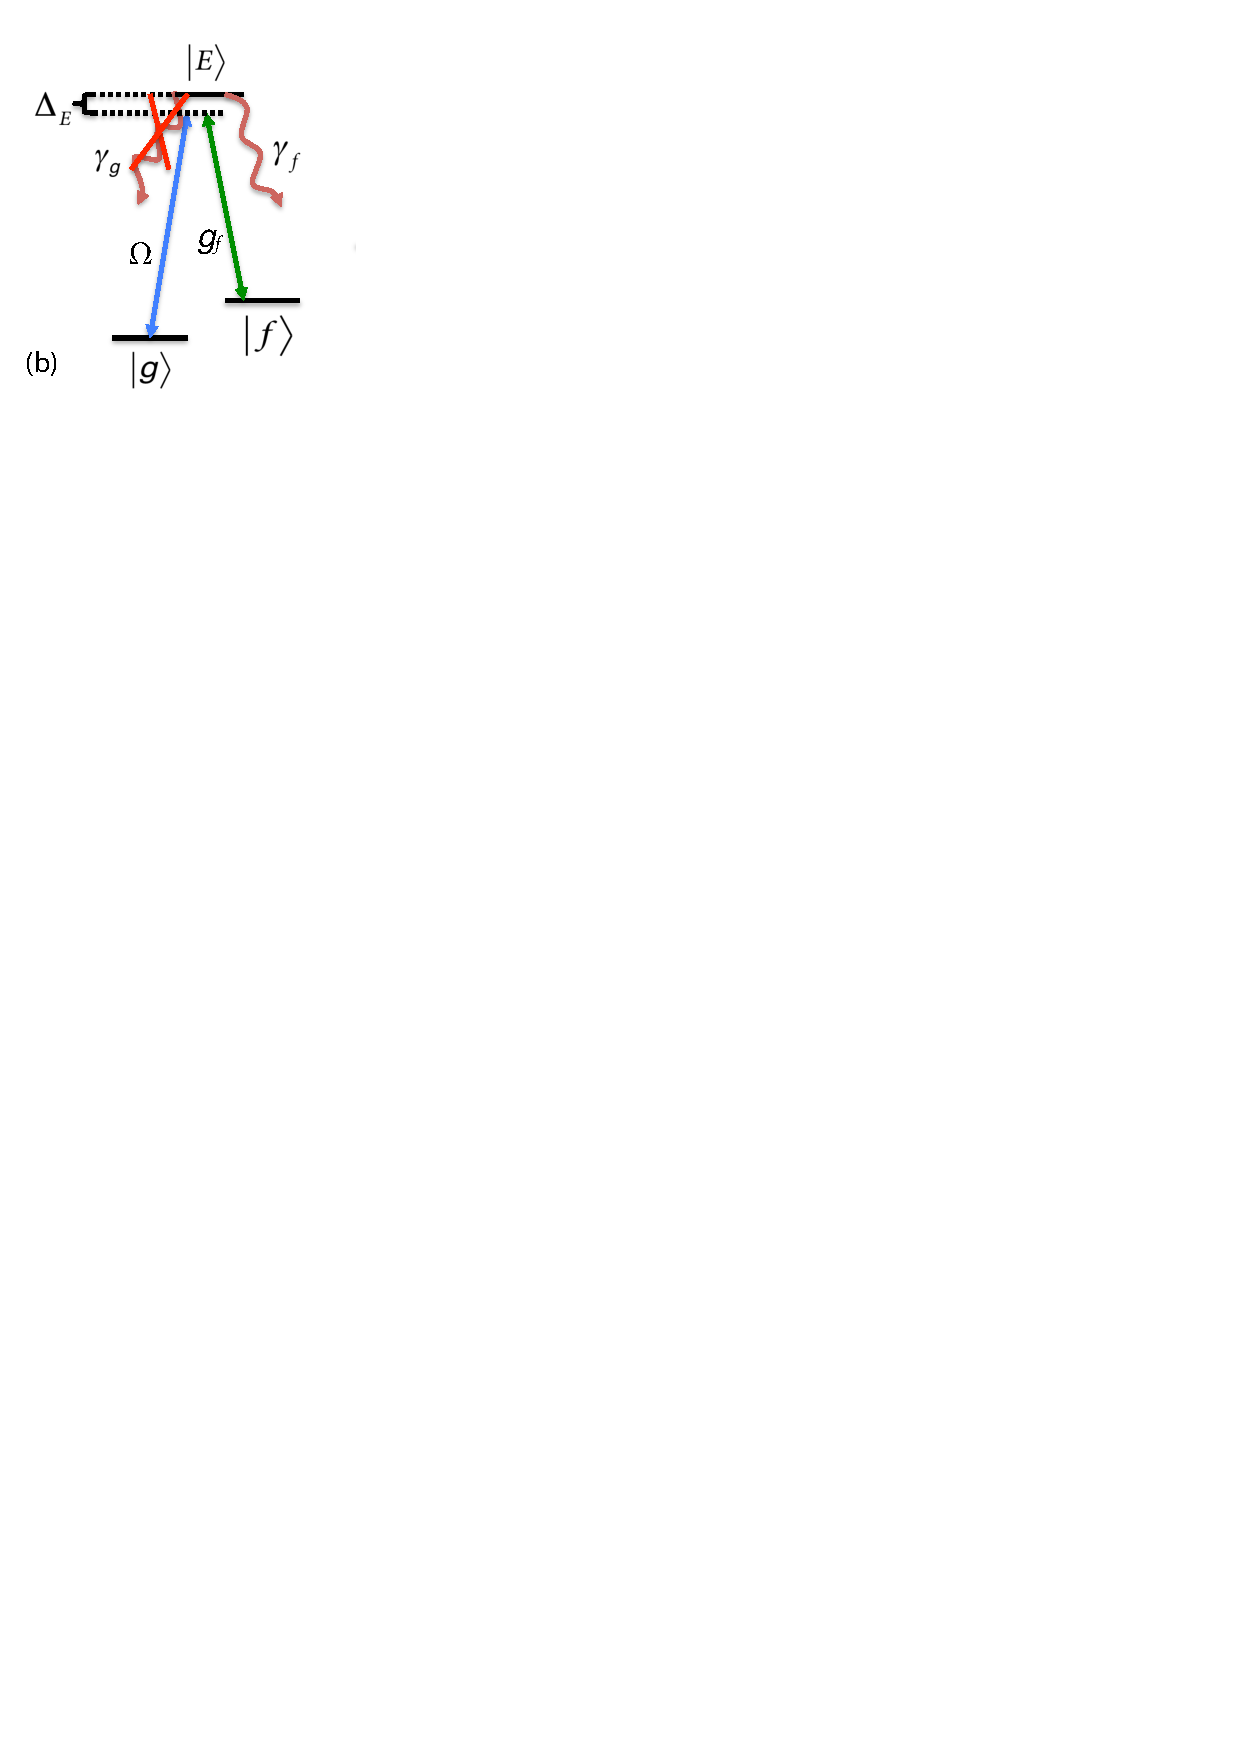
\includegraphics[width=0.35\textwidth]{./figs_Borregaard_PRL2015/figure1b}
\caption
[Level structures of qubit and control atoms]
{(a) Level structure of the qubit atoms. Only state $\ket{1}$ couples to
the cavity and we assume that the excited level decays to some level
$\ket{\tilde{o}}$, possible identical to $\ket{f}$ or $\ket{0}$. (b) Level
structure of the auxiliary atom and the transitions driven by the weak laser
($\Omega$) and the cavity ($g_{f}$). We assume that
$\ket{E}\leftrightarrow\ket{f}$ is a closed transition, i.e. $\gamma_{g}=0$.  }
\label{fig:levels}
\end{figure}

\section{Performance}

\subsection{Model}
We now analyze the performance of the gates and derive the success
probabilities, gate times and gate errors (see Tab.~S1 in Appendix
\ref{app:Borregaard_PRL2015}) The Hamiltonian in a proper rotating frame is (see
\reffig{fig:levels})
\begin{eqnarray} 
\hat{H}&=&
\Delta_{E}\ket{E}
\bra{E}+g_{f}(\hat{a}\ket{E}\bra{f}+H.c)+\hat{V}+\hat{V}^{\dagger} \nonumber \\
&&+\sum_{k}\Delta_{e}\ket{e}_{k}\bra{e}+g(\hat{a}\ket{e}_{k}\bra{1}+H.c),
\end{eqnarray}          
where $k$ labels the qubit atoms ($\hbar=1$), $2\hat{V}=\Omega\ket{E}\bra{g}$
and we have assumed that all couplings ($g,\Omega$) are real. We have defined
$\Delta_{E}=\omega_{E}-\omega_{g}-\omega_{L}$, and
$\Delta_{e}=\omega_{e}-\omega_{g}-\omega_{L}+\omega_{f}-\omega_{1}$, where
$\omega_{L}$ is the laser frequency and otherwise $\omega_{x}$ is the frequency
associated with level $x$. We describe the cavity decay and atomic spontaneous
emission with Lindblad operators so that $\hat{L}_{0}=\sqrt{\kappa}\hat{a}$
corresponds to the cavity decay,  $\hat{L}_{f}=\sqrt{\gamma_{f}}\ket{f}\bra{E}$
to the decay of the excited state of the auxiliary atom and
$\hat{L}_{k}=\sqrt{\gamma}\ket{\tilde{o}}_{k}\bra{e}$ describes the decay of the
excited qubit states to some arbitrary ground state $\ket{\tilde{o}}$. The
nature of $\ket{\tilde{o}}$ is not important for the dynamics of the gates and
it may or may not coincide with $\ket{0}$ or $\ket{1}$.

\subsection{Effective Hamiltonian}

We assume a weak driving pulse justifying for a perturbative treatment of
$\hat{V}$ using the formalism of Ref.~\cite{Florentin}. In the perturbative
description we adiabatically eliminate the coupled excited states of the atoms
and the cavity (assuming $\Omega^{2}/\Delta_{E}\!\ll\!\Delta_{E}$ and
$\Omega\!\ll\!g$), which leads to an energy shift of the ground states but
otherwise conserves them since the Hamiltonian cannot connect different
unexcited states without decay. The dynamics are therefore described by an
effective Hamiltonian,
$\hat{H}_{\text{eff}}=\ket{g}\bra{g}\sum_{n}\Delta_{n}\hat{P}_{n}$ where
\begin{equation}
\Delta_{n}=
\mathrm{Re}\left\{\frac{-\frac{\Omega^{2}}{4\gamma}
((\frac{\Delta_{e}}{\gamma}\!\!-\!\!i/2)i\!\!+\!\!2nC)}
{(2\frac{\Delta_{e}}{\gamma}\!\!-\!\!i)((2\frac{\Delta_{E}}{\gamma}
\!\!-\!\!i)i/4\!\!+\!\!C)\!\!+\!\!(2\frac{\Delta_{E}}{\gamma}\!\!-\!\!i)
nC}\right\}\label{eq:detunings}
\end{equation} 
and $\hat{P}_{n}$ projects on the states with $n$ qubits in state $\ket{1}$. For
simplicity, we have assumed that the auxiliary atom is identical to the qubit
atoms such that $g_{f}=g$ and $\gamma_{f}=\gamma$ (see Appendix
\ref{app:Borregaard_PRL2015} for a more general treatment) and we have defined
the cooperativity $C=g^{2}/\gamma\kappa$.
We consider the limit $C\gg1$ and from Eq.~\eqref{eq:detunings} we find that the
energy shift, in the case when all qubit atoms are in $\ket{0}$, becomes very
small $\Delta_{0}\sim\Delta_{E}\Omega^{2}/(16\gamma^{2} C^{2})\rightarrow 0$,
i.e., we drive into a zero energy dark state as mentioned in the description
above.
On the contrary, for $n>0$, the $C$ in the nominator of $\Delta_{n}$ reflects
that the coupling of the qubit atoms shifts the cavity resonance and as a result
an AC stark shift of $\sim\Omega^{2}/\Delta_{E}$ is introduced.
Furthermore, we find that in the effective evolution, errors caused by
spontaneous emission or cavity decay ($\hat{L}_{0},\hat{L}_{f},\hat{L}_{k}$)
project the system out of the effective space into orthogonal subspaces, which
allows for an efficient error detection by measuring the ancilla atom.

\subsection{Success probability}

The dynamics described by $\hat{H}_{\text{eff}}$ can be used to implement a
Toffoli gate. Assuming the qubit atoms to be on resonance $(\Delta_{e}=0)$ and
having $\Delta_{E}\sim\gamma\sqrt{C}$ gives energy shifts
$\Delta_{n>0}\sim\Omega^{2}/(4\gamma\sqrt{C})$ while
$\Delta_{0}\sim\mathcal{O}(\Omega^{2}/C^{3/2})$. Hence, $\ket{00...0}$ is the
only state, which remains unshifted and we can choose a gate time of
$t_{\text{T}}\sim4\pi\sqrt{C}\gamma/\Omega^{2}$ to make a Toffoli gate. By
conditioning on measuring the auxiliary atom in state $\ket{g}$ at the end of
the gate, the detectable errors from cavity decay and spontaneous emission only
reduce the success probability instead of reducing the fidelity. Consequently,
the fidelity becomes limited by more subtle, undetectable errors (see
Appendix \ref{app:Borregaard_PRL2015}). The dominant error originates from the
qubit dependent decay rate, $\Gamma_{n}$, of $\ket{g}\to\ket{f}$. As we
demonstrate in Appendix \ref{app:Borregaard_PRL2015}), this leads to a fidelity lower bounded by $1-F
\lesssim 0.3/C$, with a success probability of $P_{\text{s}} \sim 1 -
3/\sqrt{C}$. Thus is a substantial improvement over the leading error in the
case of deterministic cavity-assisted gates. For generic states, the fidelity
can even be markedly higher, and improving with increasing particle number $N$,
see Appendix \ref{app:Borregaard_PRL2015}.

In the special case of only two qubits, the Toffoli gate is referred to as a
CZ-gate, and in this case, we can even improve the gate to have an arbitrarily
small error by combining it with single qubit rotations. For the general Toffoli
gate discussed above, we needed $\Delta_e=0$ to ensure the correct phase
evolution, but making the single qubit transformations $\ket{0}\to
e^{-i\Delta_{0}t/2}\ket{0}$ and $\ket{1}\to
e^{-i(\Delta_{1}-\Delta_{0})t/2}\ket{0}$, at the end of a driving pulse of
length $t_{\text{CZ}}=\abs{\pi/(\Delta_{2}-2\Delta_{1}+\Delta_{0})}$, ensures
the right phase evolution of the CZ-gate without any constraints on
$\Delta_{e}$. Hence, it is possible to tune $\Delta_{e}$ to eliminate the
detrimental effect of having a qubit dependent decay rate. Choosing
$\Delta_{E}=\frac{\gamma}{2}\sqrt{4C+1}$ and
$\Delta_{e}=\frac{1}{2}C\gamma^{2}/\Delta_{E}$ ensures
$\Gamma_0=\Gamma_1=\Gamma_2$, and thus removes all dissipative errors from the
heralded gate. The conditional error is then limited only by non-adiabatic
effects, that can in principle be made arbitrarily small by reducing the driving
strength. The success probability is $1-P_{\text{s}}\sim 6/\sqrt{C}$ in the
limit $C\gg1$ (see \reffig{fig:prob}).
We thus have a heralded two qubit gate with arbitrarily small error with a
success probability that can approach 1 (it is possible to decrease the scaling
factor of the probability from $\sim6$ to $\sim3.4$ at the expense of an error
scaling as $1/C$ by tuning $\Delta_{E},\Delta_{e}$).

\subsection{Gate time}

We now consider the gate time. The gate time of the Toffoli gate is
$t_{\text{T}}\sim4\pi\sqrt{C}\gamma/\Omega^{2}$ and for the CZ-gate we have
$t_{\text{CZ}}\sim15\pi\sqrt{C}\gamma/(2\Omega^{2})$ for $C\gg1$. Since
$t_{\text{CZ}}>t_{\text{T}}$ we focus on $t_{\text{CZ}}$. The gate time is set
by the strength ($\Omega$) of the driving pulse, which is limited by
non-adiabatic errors. This is investigated in the supplemental material where we
also verify our analytical results numerically in Appendix
\ref{app:Borregaard_PRL2015}.
Assuming realisitc parameters of $\kappa=100\gamma$ \cite{thompson,Tiecke}, we find that a driving
of $\Omega=\sqrt{C}\gamma/4$ keeps the non-adiabatic error of the gate below
$4\cdot10^{-5}$ for $C\leq1000$. The gate times decreases as $1/\sqrt{C}$ as
shown in \reffig{fig:prob}. For a cooperativity of $100$ the gate time is
$\approx1$ $\mu$s  for typical atomic decay rates.
\begin{figure}  
\centering
$\vcenter{\hbox{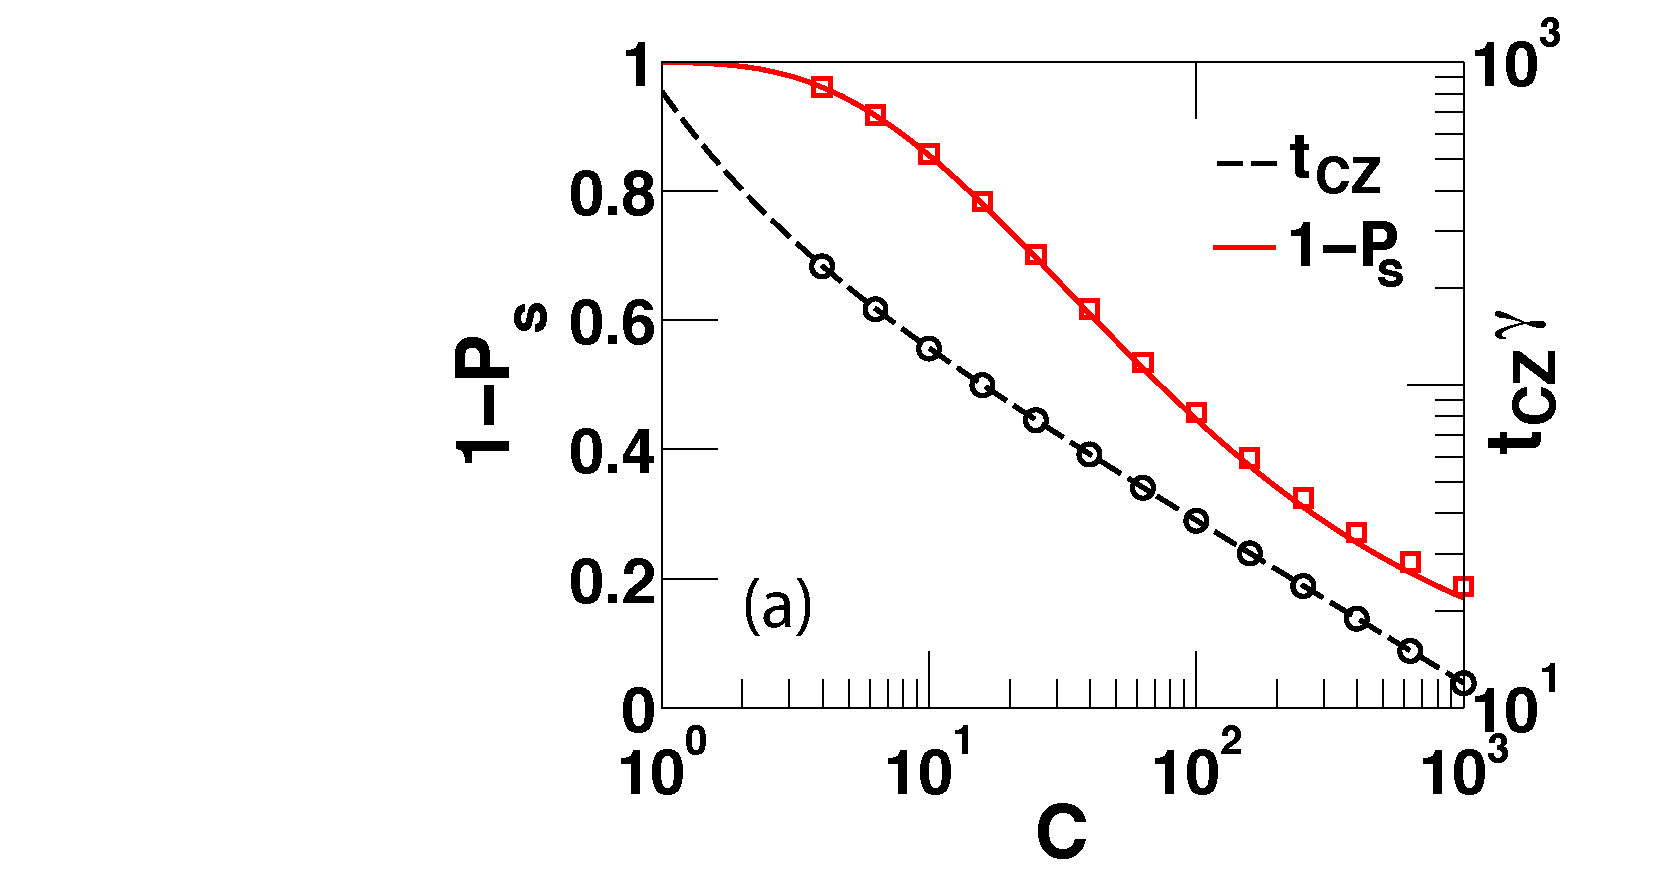
\includegraphics[width=0.45\textwidth]{./figs_Borregaard_PRL2015/figure3a}}}$
\quad\quad
$\vcenter{\hbox{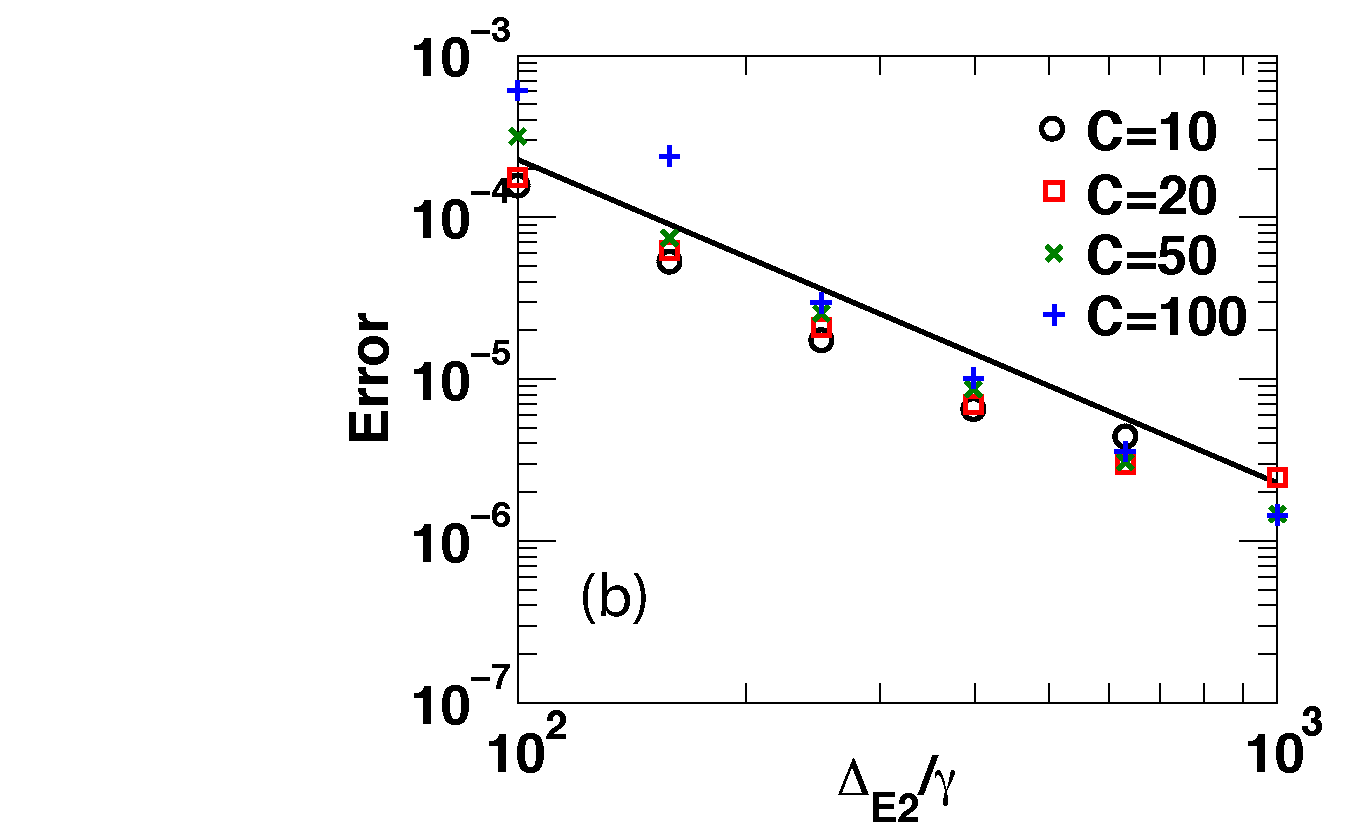
\includegraphics[width=0.45\textwidth]{./figs_Borregaard_PRL2015/figure3b2}}}$
\caption
[Success probability]
{(a) Failure probability ($1-P_{s}$ - left axis) and gate time ($t_{\text{CZ}}$
-right axis) as a function of the cooperativity ($C$) for the CZ gate. The gate
time is in units of the inverse linewidth $1/\gamma$ of the qubit atoms. We have
assumed a driving of $\Omega=\sqrt{C}\gamma/4$. (b) Gate error as a function of
the detuning $\Delta_{E2}$ in the two-photon-driven CZ-gate for $C=10,20,50$,
and $100$. We have assumed that $\Omega_{\text{\text{MW}}}=4\gamma C^{1/4}$ and
that $\gamma_{g}=\gamma$. The gate error decreases as
$\gamma^{2}/\Delta_{E2}^{2}$ and is independent of $C$.  We have assumed
$\Omega\sim\Delta_{E2}/8$ resulting in a gate time $\sim400/\gamma$.
Solid/dashed lines are analytical results and symbols are numerical simulations
(see Appendix \ref{app:Borregaard_PRL2015}). For both plots, we have assumed
$\kappa=100\gamma$.}
\label{fig:prob}
\end{figure} 

\section{Additional errors}

So far, we have assumed a model where there is no decay from
$\ket{E}\to\ket{g}$. In real atoms, there will, however, always be some decay
$\ket{E}\to\ket{g}$ with a decay rate $\gamma_{g}>0$. The result of such an
undetectable decay is that both the CZ-gate and the Toffoli gate will have an
error $\sim \gamma_{g}/(\gamma\sqrt{C})$. To make this error small, it is thus essential to suppress the
branching ratio $\gamma_{g}/\gamma$. Below we show how to suppress $\gamma_{g}$ by driving the $\ket{g}\to\ket{E}$
transition with a two photon process. As a result, we realize a CZ gate with an
error arbitrary close to zero and a Toffoli gate with an error scaling  as $1/C$
even for a realistic atomic system.

Specifically we think of a level structure for the auxiliary atom, shown in
\reffig{fig:control},
\begin{figure} 
\centering
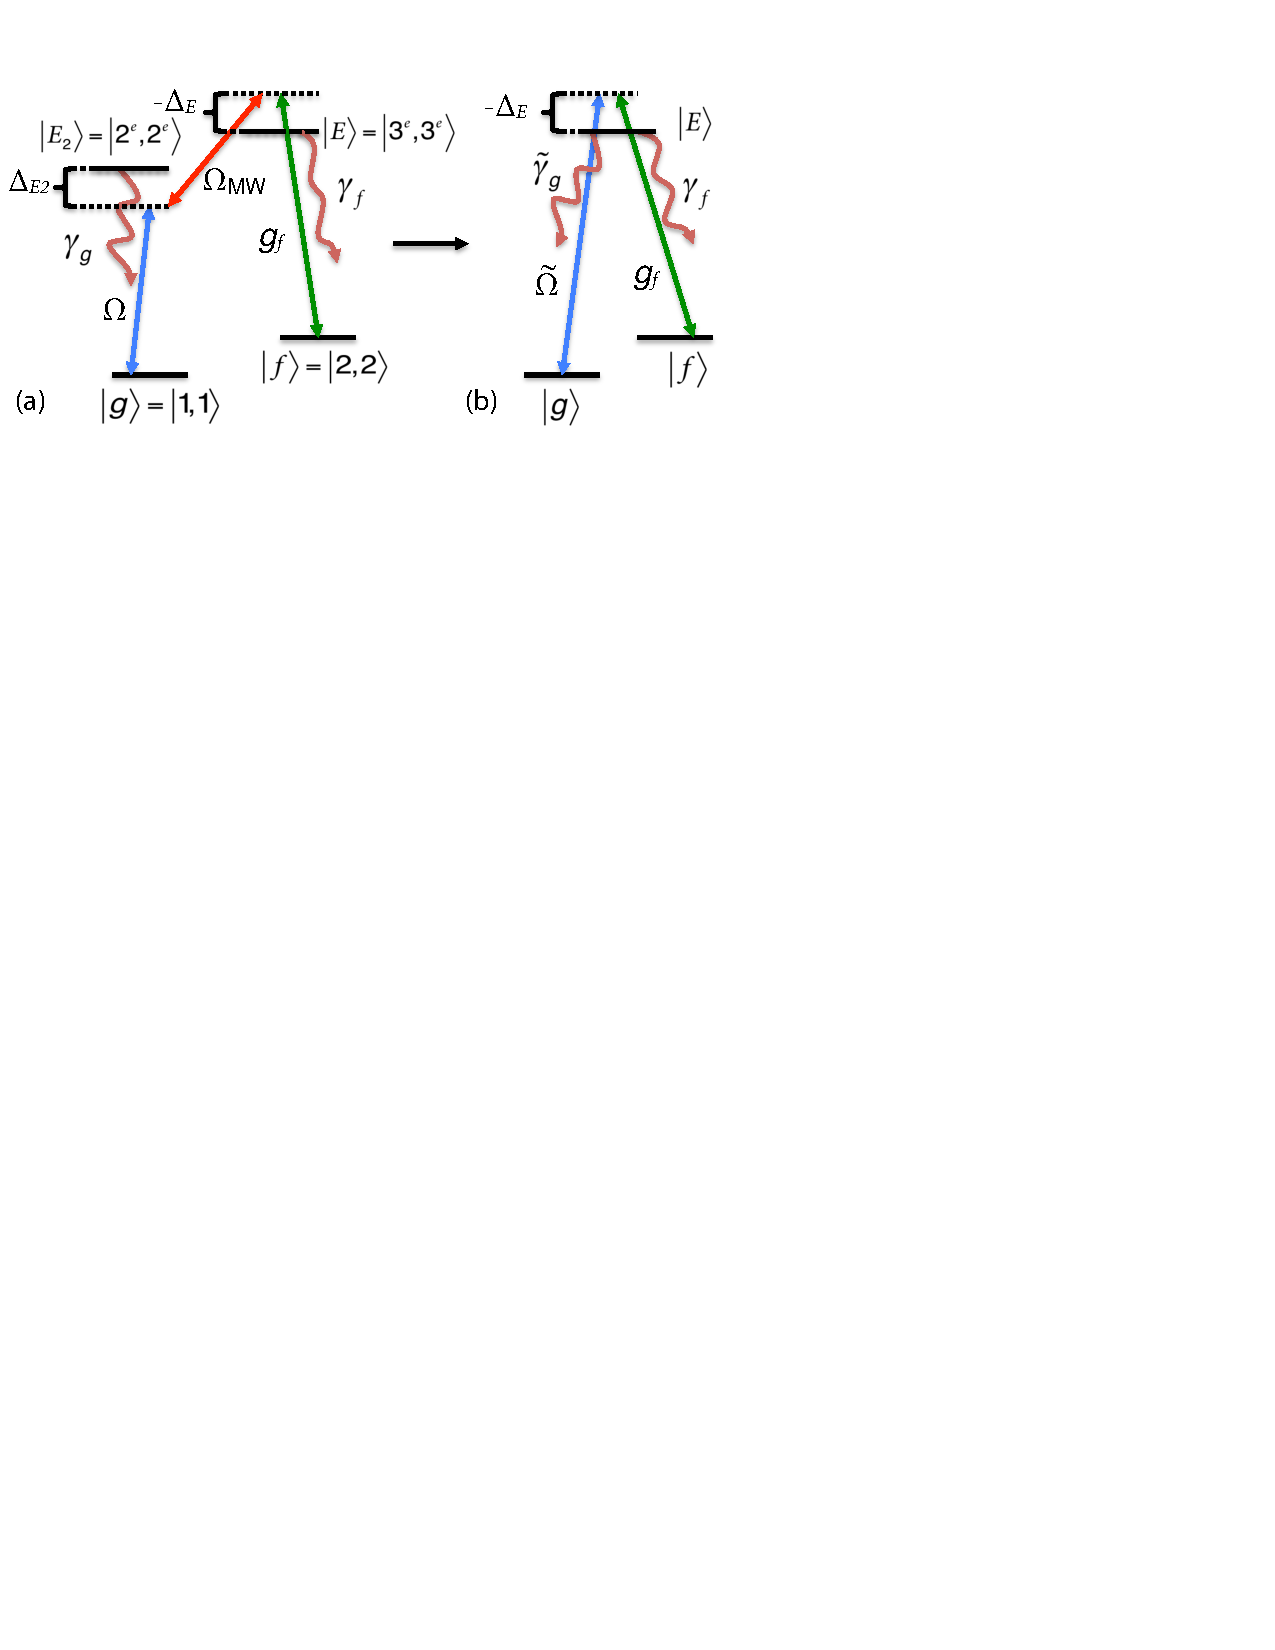
\includegraphics[width=0.75\textwidth]{./figs_Borregaard_PRL2015/figure4}
\caption
[Level structure of auxiliary atom]
{(a) Level
structure of the auxiliary atom and the transitions driven by a weak laser ($\Omega$), a microwave field ($\Omega_{\text{MW}}$) and the cavity ($g_{f}$). We assume that
$\ket{E}\leftrightarrow\ket{f}$ is a closed transition and, for simplicity, we
also assume that $\ket{E_{2}}\leftrightarrow\ket{g}$ is a closed transition but
this is not a necessity. Here $\ket{r^{(e)},r^{(e)}}$ with $r=1,2,3$ refers to
how the atom may be realized in the $(5^{2}P_{3/2})$ states
$\ket{F^{(e)}=r,m^{(e)}=r}$ $5^{2}S_{1/2}$ of Rb${}^{87}$. (b) Effective
three-level atom realized by mapping the two-photon drive to give an effective
decay rate $\tilde{\gamma}_{g}$ and an effective drive $\tilde{\Omega}$. }
\label{fig:control}
\end{figure} 
where we still assume $\ket{E}\leftrightarrow\ket{f}$ to be a closed transition.
For simplicity, we have also assumed $\ket{E_{2}}\leftrightarrow\ket{g}$ to be a
closed transition. Such a level structure could,
e.g. be realized in  ${}^{87}$Rb  as shown in \reffig{fig:control}.  We assume
that a microwave field couples the two excited states such that we can have a
two photon transition from $\ket{g}\to\ket{E}$ and that $\Omega$ is small,
allowing for a perturbative treatment of the coupling. Thus we can map
the system to a simple three-level atom with levels $\ket{g},\ket{E}$ and
$\ket{f}$ and a decay rate $\tilde{\gamma}_{g}$ and drive $\tilde{\Omega}$
between $\ket{g}$ and $\ket{E}$, determined by the two photon driving process as
shown in \reffig{fig:control}. The dynamics are thus similar to what we have
already described for the simple three level atom except that we have the extra
decay $\tilde{\gamma}_{g}$ that introduces an error in the gates
$\sim(\tilde{\gamma}_{g}/\gamma)/\sqrt{C}$, as previously described. In the
limit $C\gg1$, we find
$\tilde{\gamma}_{g}/\gamma\sim\frac{\gamma_{g}\Omega_{\text{MW}}^{2}}{4\gamma\Delta_{E2}^{2}}$.
Thus by increasing $\Delta_{E2}$, we can in principle make these errors
arbitrarily small. The error of the CZ-gate for different $\Delta_{E2}$ is shown
in \reffig{fig:prob}, assuming an initial state of
$(\ket{0}+\ket{1})^{\otimes 2}$. Note that in order to prevent an increasing
scattering probability of level $\ket{E2}$, we need to have $\Omega_{MW}\propto
C^{1/4}$ resulting in a gate error that is independent of the cooperativity, see
Appendix \ref{app:Borregaard_PRL2015}.
The success probability and time of the gates are the same as before with
$\Omega\to\tilde{\Omega}\sim\frac{\Omega_{\text{MW}}\Omega}{2\Delta_{E2}}$. With
similar considerations about the validity of our perturbation as
before, we find that for realistic parameters, we can use $\Omega=\Delta_{E2}/8,
\Omega_{\text{MW}}\sim4\gamma C^{1/4}$ resulting in a gate time of $\sim10$
$\mu$s for typical atomic decay rates and $C\lesssim1000$, see Appendix
\ref{app:Borregaard_PRL2015}.

\section{Possible implementation}

As an example implementation, we consider ultra-cold ${}^{87}$Rb atoms coupled
to nanophotonic cavities~\cite{thompson,Tiecke}. There are some additional
errors originating from the extra states in the ${}^{87}$Rb atoms in this case.
In Appendix \ref{app:Borregaard_PRL2015}, we treat these errors and find that with a detuning of
$\Delta_{E2}=100\gamma$ and a cooperativity of $C\approx100$, a heralded CZ gate
with $\sim67\%$ success probability and a heralded error of $\approx 10^{-3}$
can be realized in $\approx10$ $\mu$s time. This justifies neglecting atomic
decoherence which is typically much slower.
Alternatively the gate can be implemented with atom-like solid-state qubits such
as NV and SiV centers in diamond~\cite{phystoday}. These systems can exhibit
closed transitions and long-lived electronic spin states which are the essential
requirement for the gate~\cite{togan}, while high cooperativities are possible
in  diamond nanocavities~\cite{burek}. A particular advantage of such system is
the long-lived nuclear spin degrees of freedom, which allows each of the color
centers  to act as a multi-qubit quantum network node~\cite{maurer}.   By
entangling electronic spins via the heralded gate, a high-fidelity, fully
deterministic gate can subsequently be performed on qubits stored in nuclear
spins~\cite{Anders2prl}.

\section{Application}

As a particular application, we consider a quantum repeater where entanglement
is first created in small segments (links), which are subsequently connected
using entanglement swapping~\cite{briegel}. By organizing the repeater in a tree
structure, the probabilistic nature of the gate can be efficiently circumvented.
The success rate of distributing entanglement across the total distance L,
scales as $\sim (L/L_{0})^{1-\log_{2}(3/p)}$, where $p<1$ is the success
probability of the swap, $L$ is the total distribution distance and $L_{0}$ is
the length between the links~\cite{Borregaard2015b} (note that in the limit $p\to1$,
the above expression underestimates the rate, e.g., for $p=1$ the actual rate is
$\sim3$ times faster for 128 links). This is a substantial improvement over
direct transmission where the success rate scales exponentially with $L$. For a
realization with nuclear spin memories where the swap can be performed
deterministically the rate can scale even better as
$\sim\log_{2}(L/L_{0})^{-1}$. In order to maintain the favorable scaling without
resorting to time consuming purification, the total number of links,
$N_{\text{max}}$ should be kept below
$N_{\text{max}}\sim-\ln(F_{\text{final}})/(\epsilon_{0}+\epsilon_{g})$, where
$F_{\text{final}}$ is the required fidelity of the final distributed pair and
$\epsilon_{0},\epsilon_{g}\ll1$ are the errors of the initial entanglement
generation and the entanglement swapping respectively. Thus, it is essential
that the errors are kept small, which can be obtained with the heralded gate.

\section{Conclusion}

In conclusion, we have introduced a heralded two-qubit quantum
gate with a conditional fidelity arbitrarily close to unity and an $N$-qubit Toffoli gate
with an error scaling as $1/C$. The gates have a
built-in error detection process, which removes the necessity of extracting the
error by the more complicated process of entanglement purification or quantum
error correction. Our gate is designed for the specific case of optical
cavities, and allows exploiting realistic systems for quantum communication, even though the error rate would inhibit this with deterministic gates. Similar
advantages can be realised in other systems such as those based on circuit QED, where certain errors could be
heralded and thus alleviate the daunting requirements of fault tolerant
computation. 
